\documentclass[12pt, a4paper, simple]{eskdtext}

\usepackage{hyperref}
\usepackage{env}
\usepackage{_sty/gpi_lst}
\usepackage{_sty/gpi_toc}
\usepackage{_sty/gpi_t}
\usepackage{_sty/gpi_p}
\usepackage{_sty/gpi_u}

% Код
% \ESKDletter{О}{Л}{Р}
% \def \gpiDocTypeNum {81}
% \def \gpiDocVer {00}
% \def \gpiCode {\ESKDtheLetterI\ESKDtheLetterII\ESKDtheLetterIII.\gpiStudentGroupName\gpiStudentGroupNum.\gpiStudentCard-0\gpiDocNum~\gpiDocTypeNum~\gpiDocVer}

\def \gpiDocTopic {Отчёт лабораторной работы №\gpiDocNum}

% Графа 1 (наименование изделия/документа)
% \ESKDcolumnI {\ESKDfontII \gpiTopic \\ \gpiDocTopic}

% Графа 2 (обозначение документа)
% \ESKDsignature {\gpiCode}

% Графа 9 (наименование или различительный индекс предприятия) задает команда
% \ESKDcolumnIX {\gpiDepartment}

% Графа 11 (фамилии лиц, подписывающих документ) задают команды
% \ESKDcolumnXIfI {\gpiStudentSurname}
% \ESKDcolumnXIfII {\gpiTeacherSurname}
% \ESKDcolumnXIfV {\gpiTeacherSurname}

\begin{document}
    \begin{ESKDtitlePage}
    \ESKDstyle{empty}
    \begin{center}
        \gpiMinEdu \\
        \gpiEdu \\
        \gpiKaf \\
    \end{center}

    \vfill

    \begin{center}
        \gpiTopic
    \end{center}

    \vfill

    \begin{center}
        \textbf{\gpiDocTopic} \\
        ПО ДИСЦИПЛИНЕ \gpiDiscipline \\
    \end{center}

    \vfill

    \begin{flushright}
        \begin{minipage}[t]{7cm}
            Выполнил:\\
            \PageTitleStudentInfo
            \PageTitleDateField
            \hspace{0pt}

            Проверил:\\
            \PageTitleTeacherInfo
            \PageTitleDateField
        \end{minipage}
    \end{flushright}

    \vfill

    \begin{center}
        \PageTitleCity~\ESKDtheYear
    \end{center}
\end{ESKDtitlePage}

    \ESKDstyle{empty}
    \begin{center}
        \textbf{\gpiDocTopic}
    \end{center}

    % = = = = = = = =
    \paragraph{} \textbf{Тема}: <<\gpiTopicRep>>

    \paragraph{} \textbf{Цель}: реализовать Android приложение, которое работает с JSON форматом.

    \paragraph{} \textbf{Что нужно сделать}:

    Реализовать отображение списока элементов внутри фрагмента ListView.
    Cписок занимает более одного экрана, то есть список можно пролистать.
    Реализовать отдельный элемент списка с пользовательским стилем/дизайном (user\_item.xml).
    Выполнять запрос на получение данных с удаленного сервера, используя AsyncTask.
    Выполнять преобразование json-структуры (JSONObject, JSONArray) в коллекцию объектов (список - ArrayList, карт - HashMap).

    \paragraph{} \textbf{Разработка дизайна}:

    \begin{figure}[!h]
        \centering
        \begin{minipage}{0.49\textwidth}
            \centering
            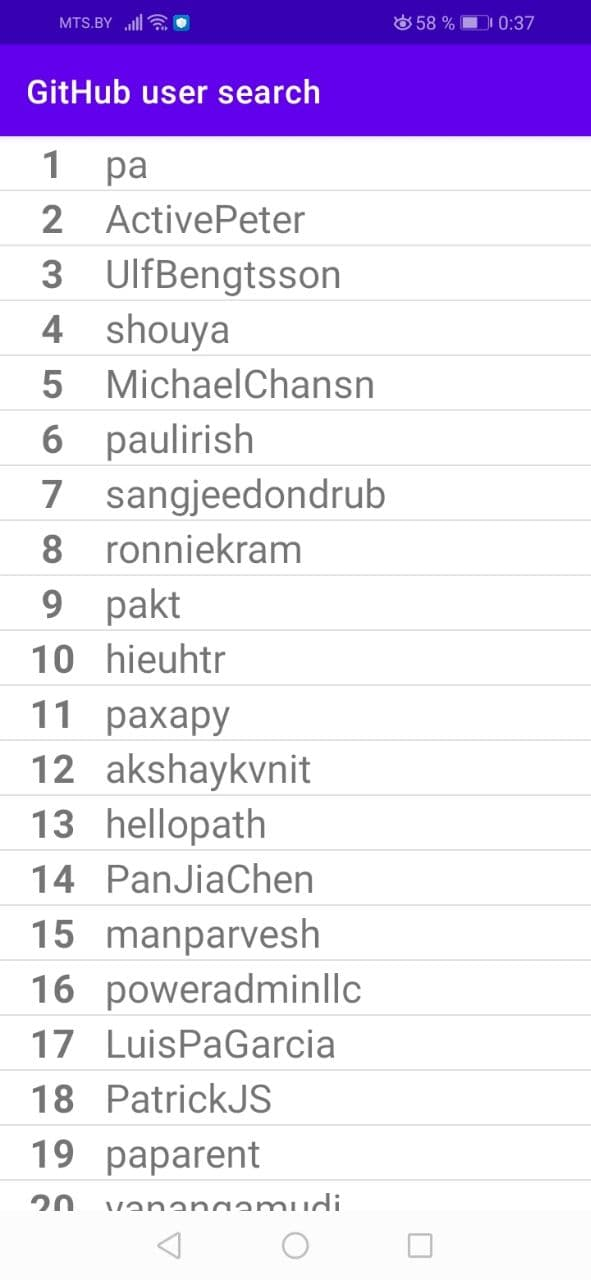
\includegraphics[height=12cm]
                {_assets/top.jpg}
            \caption{Верхушка списка}
            \label{fig:gpi_start}
        \end{minipage}
        \begin{minipage}{0.49\textwidth}
            \centering
            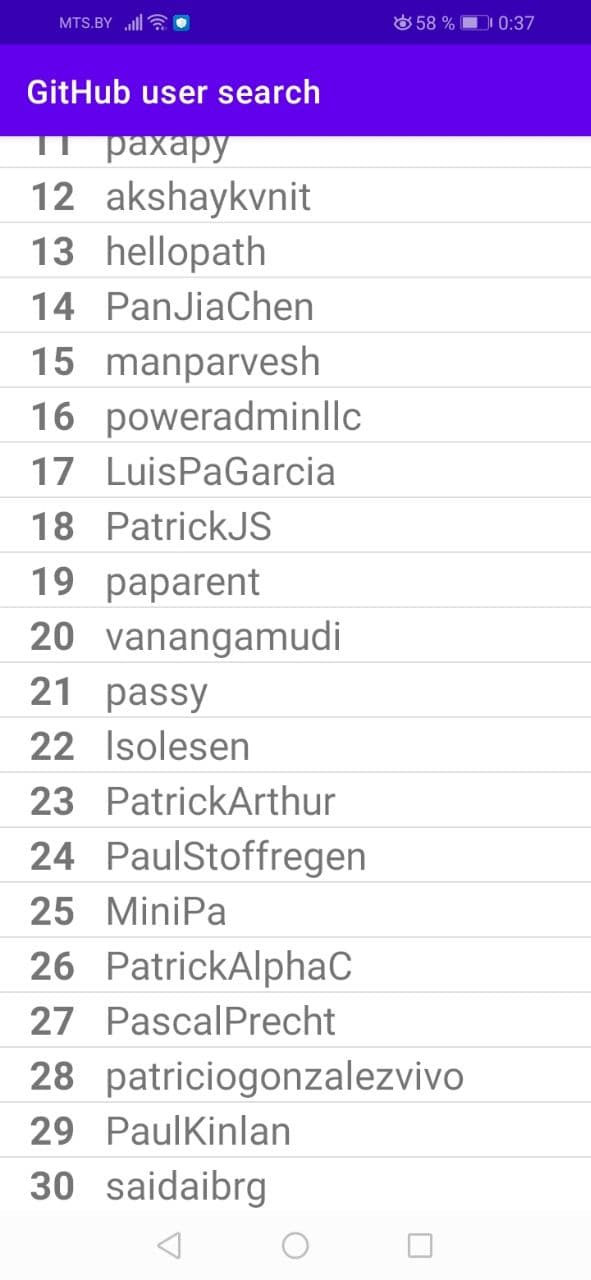
\includegraphics[height=12cm]
                {_assets/bottom.jpg}
            \caption{Прокрутили список}
            \label{fig:gpi_behind}
        \end{minipage}
    \end{figure}


    \newpage
    \paragraph{} \textbf{Исходный код}: 

    \lstinputlisting[language=java, name=app/src/main/java/.../MainActivity.java]
        {../gpi_src/gpi_rpodms6_lab5/app/src/main/java/io/github/Pavel_Innokentevich_Galanin/gpi_rpodms6_lab5/MainActivity.java}

    \lstinputlisting[language=xml, name=app/src/main/AndroidManifest.xml]
        {../gpi_src/gpi_rpodms6_lab5/app/src/main/AndroidManifest.xml}

    \lstinputlisting[language=xml, name=app/src/main/res/values/strings.xml]
        {../gpi_src/gpi_rpodms6_lab5/app/src/main/res/values/strings.xml}
    
    \lstinputlisting[language=xml, name=app/src/main/res/layout/activity_main.xml]
        {../gpi_src/gpi_rpodms6_lab5/app/src/main/res/layout/activity_main.xml}

    \lstinputlisting[language=xml, name=app/src/main/res/layout/user_item.xml]
        {../gpi_src/gpi_rpodms6_lab5/app/src/main/res/layout/user_item.xml}

    \paragraph{} \textbf{Вывод}:
    Реализовали отображение списока элементов внутри фрагмента ListView.
    Cписок занимает более одного экрана, то есть список можно пролистать.
    Реализовали отдельный элемент списка с пользовательским стилем/дизайном (user\_item.xml).
    Выполняли запрос на получение данных с удаленного сервера, используя класс AsyncTask.
    Выполняли преобразование json-структуры (используя классы JSONObject и JSONArray) в коллекцию объектов (используя классы ArrayList и HashMap).

    % = = = = = = = =
    \paragraph{} \textbf{Список использованных источников}:
    % \addcontentsline{toc}{section}{СПИСОК ИСПОЛЬЗОВАННЫХ ИСТОЧНИКОВ}
    % \section*{Список использованных источников}
    \begin{enumerate}
        \item[1.] Изучение Android Studio за час в одном видео! Создание погодного приложения с API - YouTube  [Электронный ресурс]
        - Режим доступа: \url{https://www.youtube.com/watch?v=zzV2aML_zNg}.
        Дата~доступа:~23.02.2022.

        \item[2.] Уроки Android Studio с нуля / \#11 – Обработка массивов данных (ListView) - YouTube  [Электронный ресурс]
        - Режим доступа: \url{https://www.youtube.com/watch?v=OamuOYuLiIQ}.
        Дата~доступа:~23.02.2022.

        \item[3.] Android Studio: получение JSON в RecyclerView и CardView. Урок № 1 - YouTube  [Электронный ресурс]
        - Режим доступа: \url{https://www.youtube.com/watch?v=BKnn5QeJ7WU}.
        Дата~доступа:~23.02.2022.

        \item[4.] Android Studio: получение JSON в RecyclerView и CardView. Урок № 1  [Электронный ресурс]
        - Режим доступа: \url{https://maxfad.ru/programmer/android/671-android-studio-poluchenie-json-v-recyclerview-i-cardview-urok-1.html}.
        Дата~доступа:~23.02.2022.

        \item[5.] Parsing JSON from URL into ListView - [JSON Parsing Course \#5] - YouTube  [Электронный ресурс]
        - Режим доступа: \url{https://www.youtube.com/watch?v=v4X0y6-VOtM}.
        Дата~доступа:~23.02.2022.
    \end{enumerate}
    \newpage
\end{document}
